\section{Deep learning}
\label{sec:deep_learning}

As with many computer science subfields deep learning has outperformed manual feature engineering on many NLP tasks.
For the last few years the best performing NLP systems have been neural networks.
This section will provide a basic overview of the most important model architectures.
Importance is decided by seeing what is mentioned often when reading about NLP and looking at the state-of-the-art at the time of writing.
So, completeness of this discussion is not guaranteed.

% TODO: Explain encoder decoder.
% TODO: Explain transfer learning? (used for ELMo)

\subsection{word2vec}
\label{subsec:word2vec}


\iffalse
This section will take one step in the direction of using deep learning for NLP.
Neural networks are basically a mapping from vector to vector (numbers to numbers).
Natural language can be converted from and to vectors using embeddings.
This section will introduce embeddings and explain some common concepts.
The focus lies on the intuition behind the approaches.
The goal of this is being able to estimate suitability of certain approaches for certain tasks.
\fi

\subsection{glove}
\label{subsec:glove}


\subsection{Vanishing gradient problem}
\label{subsec:vanishing_gradient_problem}
The vanishing gradient problem has for a long time halted the progress of neural networks with many layers, also known as deep neural networks.
The problem relates to vanishing and exploding updates to weights in the earlier layers.
These extreme updates are caused by the backpropagation.
Consider some weight $w$ which is at the front of some network.
Lets say this weight is updated by the following partial derivative $w = d_1 \cdot d_2 \cdot \ldots \cdot d_i$.
Here $i$ denotes the number of layers in the network.
These partial derivatives $d_x$ can become small $(0 \leq d_x < 1)$ or large $(1 \ll d_x)$.
Typically the learning rate has an order of magnitude of \num{1e-3}.
When one derivative is small the weight update when multiplied by learning rate might become very small.
Conversely when one derivative is big the update might become very big.
Since the weight is at the front of a deep network $i$ is big.
Thus, the chance that weights in the front vanish or explode increase by increment of $i$.
Effectively the problem causes layers which are have a long distance from the prediction layer to stop learning.

\subsection{Recurrent neural networks}
\label{subsec:rnn}
\begin{figure}[htbp]
    \begin{center}
        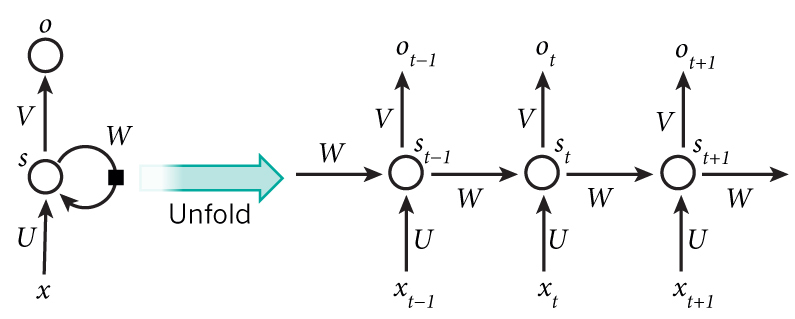
\includegraphics[width=0.5\textwidth]{figures/rnn.jpg}
    \end{center}
    \caption{Recurrent neural network~\cite[Figure 5]{lecun2015deep}.}
    \label{fig:rnn}
\end{figure}
A recurrent neural network (RNN) is an extension on neural networks which allows the network to have memory.
Simply put the network remembers a summary of information from all previous states.
A common way to visualize this is depicted in figure~\ref{fig:rnn}.
On the right side the model is unfolded in time.
The unfolded representation shows the state of the network and the flow of information for three consecutive points in time.
To access this history the neural network in current state $s_t$ obtains a `summary' from the previous state $s_{t-1}$.
Suppose we are training a RNN in an unsupervised way.
The model trains on real-world texts.
For each word $w_i$ it is asked to predict $w_i$ based only on previous words $w_1, w_2, \ldots, w_{i-1}$.
In the image $w_i$ is denoted as input $x_i$.
After predicting the prediction is compared to the correct word, if these are not equal the loss is backpropagated.
The backpropagation is then able to `change history' to improve prediction accuracy.

The benefit of this architecture over n-grams is that the information is compressed inside the neural network.
Also, there is a certain sense of importance since the weights are not uniformly updated for all previous states (words).
Take, for example, `the car, which is green, broke'.
For this sentence the word `broke' can more easily be predicted based on `the car' than on `which is green'.

In practice RNNs are not using the complete history.
The cause for this are vanishing and exploding gradients.
Solving explosions can be done by putting a threshold on the updates~\citep{mikolov2014learning}.
The vanishing gradients are harder to solve because these updates do not `jump out'.
In practise gradients still vanish and simple RNNs become like 7-grams for most words~\citep{manning2017lectures}.
This is clearly not enough.

\subsection{Gated recurrent units}
\label{subsec:gru}
Basic RNNs do not yet provide a way to translate languages.
Machine translation requires to convert some sentence from a source language to a target language.
To this end a RNN encoder-decoder has been proposed by~\citet{cho2014learning}.

\begin{figure}[htbp]
    \begin{center}
        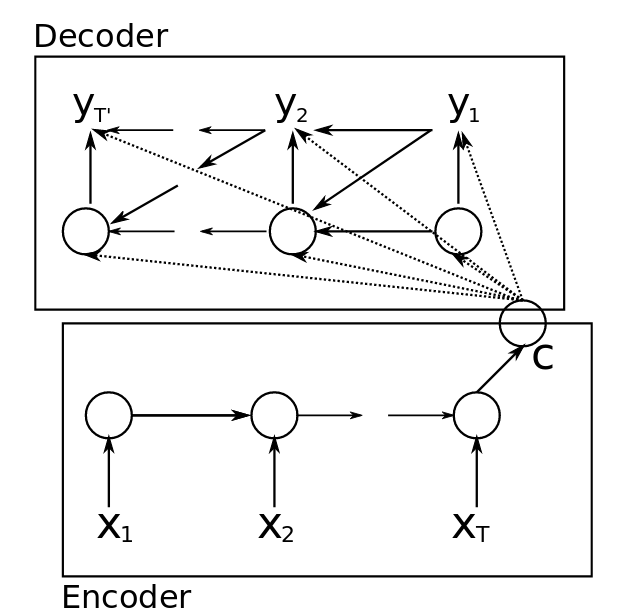
\includegraphics[width=0.5\textwidth]{figures/encoder_decoder.png}
    \end{center}
    \caption{RNN Encoder-decoder~\cite[Figure 1]{cho2014learning}.}
    \label{fig:encoder_decoder}
\end{figure}

Similar to the basic RNN the decoder at some time has access to only the previous state, see figure~\ref{fig:encoder_decoder}.
The encoder takes the source sentence of variable length $T$ and maps it to a fixed length vector.
The decoder in turn maps the fixed length vector to the target sentence of length $T'$.
To do this the network reads all words $x_1, x_2, \ldots, x_T$ until an end of line token is received.
At that point the entire sentence is captured in the hidden state $C$.
The decoder starts generating words $y_1, y_2, \ldots, y_{T'}$ based on the previous decoder states and $C$.
This is visualised by the arrows.
The authors of the paper recognized that this approach has the same limitations as the basic RNN.
Typically words in translation sentence pairs are somewhat aligned, as described in subsection~\ref{subsec:mt}.
For example, when generating the first word $y_1$ the algorithm mainly needs info from $x_1$, but has more recently seen the next words in the sequence $x_2, x_3, \cdots, x_{T'}$.
Vanishing gradients will cause the network to forget its far history, so this methods does not work well for long sentences.
To solve this the authors have also introduced gates to RNNs.

\begin{figure}[htbp]
    \begin{center}
        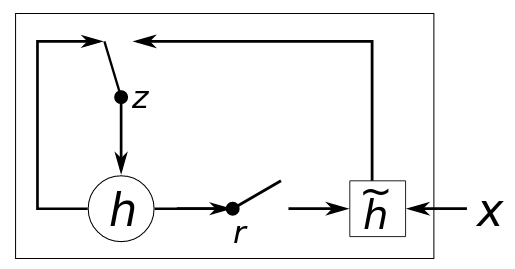
\includegraphics[width=0.5\textwidth]{figures/gru.png}
    \end{center}
    \caption{RNN Encoder-decoder~\cite[Figure 2]{cho2014learning}.}
    \label{fig:gru}
\end{figure}

Gated recurrent units have gates which automatically learn to open and close for some hidden state $h$.
The update gate $z$ whether backpropagation should be applied to $h$.
The reset gate $r$ decides whether the p

TODO: Really draw this out.
GRU intuition slide is nice.
It explains that if reset is close to 0 the previous hidden state is ignored.

\subsection{Long short term memory networks}
\label{subsec:lstm}

The encoder goes through different states until the end of line is reached.
After this the decoder uses the final state to generate the next sentence (for example, a translated sentence).
Seq2Seq?
See also CS224n.

\subsection{Attention}
\label{subsec:attention}
See also CS224n including 'advanced attention' slides.

One drawback of recurrent neural networks is that the decoder has all information from the final state of the encoder.
A problem with this can be explained by looking at machine translation.
When translating one will find that similar words often appear at similar places in sentences.
TODO: Insert alignment image and paper from slides.
This is called alignment.
When generating the $n$-th word during decoding information we generally need mainly information from the $n$-th word which occurred during encoding.
It makes more sense to focus the neural network \textit{attention} on the part of the sentence we actually need the most.
To this end the neural net learns to choose what hidden states are important.
TODO: Really add image here just like slides.
The important states get a higher weight which yield a context vector.
TODO: Way too short, need to explain better.

\subsection{Bidirectional recurrent neural networks}
\label{subsec:bidirectional}
All recurrent architectures described above use only the information on the left of some word to predict it.
Take for example the following sentences containing the polyseme `drinking'.
\begin{center}
    Peter was drinking after a workout.\\[3mm]
    Peter was drinking excessively.
\end{center}
The meaning of the word `drinking' changes after reading the next words in the sentence.
To take this into account bidirectional recurrent neural networks (BRNN) have been developed by~\citet{schuster1997}.
A BRNN contains two separate RNNs as depicted in figure~\ref{fig:bidirectional}.
The paper only considers RNNs, but the method can be applied to gated recurrent models as well.
One RNN goes through elements of the sequence from left to right and the other in the reverse direction.
Training can be done by showing the network all words except for one.
Both networks learn to predict the next word given a sequence of words.
Calculating the loss is done by taking the average of the predictions of both RNNs.
To reduce required computational power one simplification is used.
Suppose we want to learn from the word at location $k$, $w_k$.
A solution would be to get all the way to states $s_{k-1}$ and $s_{k+1}'$ to predict $w_k$.
Then we update the weights and, assuming we go forward, now want to learn from $w_{k+1}$.
The RNN in state $s_{k-1}$ takes one step forward, but the RNN in state $s_{k+1}'$ has to restart from the last word in the sequence.
To solve this both RNNs make one prediction for each word and the answers of both for the entire sequence are used to update the weights.

\begin{figure}[htbp]
    \begin{center}
        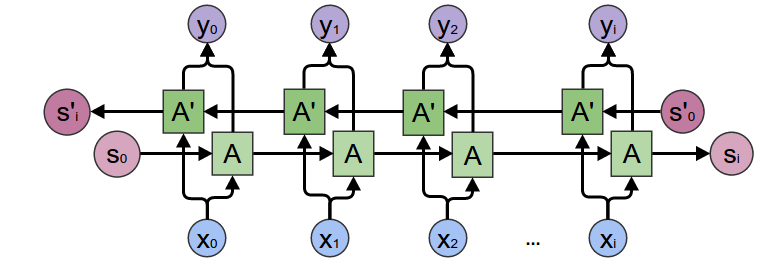
\includegraphics[width=0.5\textwidth]{figures/bidirectional.png}
    \end{center}
    \caption{Bidirectional RNN~\citep{olah2015}.}
    \label{fig:bidirectional}
\end{figure}


\subsection{Convolutional neural networks}
\label{subsec:cnn}
% cnn intro

% cnn outro
A review by~\citet{young2018recent} argues that CNNs are suited for specific NLP tasks.
However, when data is scarce they are not effective.
Foundational problems with CNNs are that they are unable to model long-distance contextual information and preserving sequential order.
The former means that CNNs are not well suited for question answering tasks.
Interestingly, this paper mentions ``BERT surpass ELMo to establish state-of-the-art in multiple tasks''.

\subsection{Transformers}
\label{subsec:transformers}
The main issue in the recurrent approaches is that distant information needs to pass through all the intermediate states.
In the basic RNN for each state all the information is updated, causing less recent information to gradually disappear.
The GRU and LSTM reduce this problem by being more selective when viewing or changing information.
In \textit{attention is all you need}~\citep{vaswani2017attention} a new approach is presented.
Instead of making a prediction on the previous state the network is allowed to make a prediction based on a large number of previous inputs.
For example, suppose we are translating `impounded' in the following sentence pair from the WMT'14 English-German dataset.
\begin{center}
    The motorcycle was seized and \underline{impounded} for three months.\\[3mm]
    Das Motorrad wurde sichergestellt und f\"ur drei Monate \underline{beschlagnahmt}.
\end{center}
Suppose the system has correctly predicted the German sentence up to and including `Monate'.
The next step is to predict `beschlagnahmt'.
To do this the system needs mainly information about the word `impounded'.
Gated recurrent architectures learn to look at the previous state in such a way that the attention is focused on `impounded'.
This requires the information of the word to not been overwritten during execution.
Transformers evade this overwriting problem by allowing the system to see all $d$ previous words, where $d$ is 1024 for the biggest model.
The only thing the transformer then needs to learn is where to focus its attention.
The information of all the previous words is stored in an array of word vectors (a tensor).
To apply focus to parts of this tensor the model learns to put a mask over the tensor.
In the mask zeroes correspond to hidden items.
One drawback is the required computational power.
Suppose we only need one word from the $d$ previous words.
The mask will hide $d-1$ words.
This still requires to multiply the masked word vectors by zero.
Google argues that this is not really an issue since matrix multiplication code is highly optimized and graphic processing units (GPUs) exist.
So, the model can relate any dependency in constant time when the range is lower than $d$.
This in contrast to recurrent layers which are in linear time.
When the sequence length is greater than $d$ computations will require more than linear time.

Another benefit of the transformers are that self-attention visualisations can more easily be done than in recurrent architectures.
By self-attention the authors refer to attention that is used to generate context aware word representations.
An example of a tranformer model correctly applying coreference resolution is presented shown in figure~\ref{fig:coreference_resolution}.

\begin{figure}[htbp]
    \begin{center}
        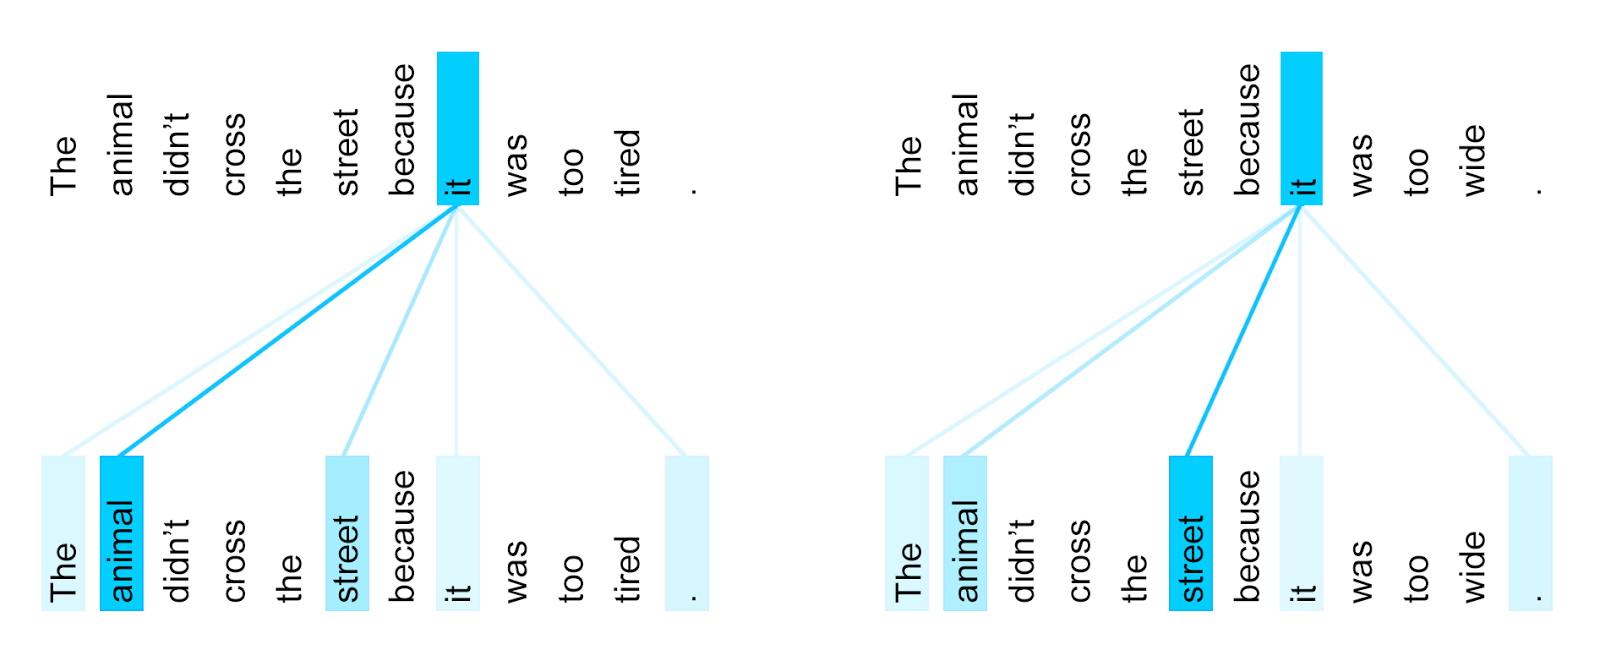
\includegraphics[width=\textwidth]{figures/coreference_resolution.png}
    \end{center}
    \caption{Encoder self-attention distribution~\citep{uszkoreit2017}.}
    \label{fig:coreference_resolution}
\end{figure}

\subsection{ELMo}
\label{subsec:elmo}
Word embeddings generated by systems such as Word2vec and GloVe do not take context into account when determining word representations.
For ELMo ``each token is assigned a representation that is a function of the entire input sentence''~\citep{peters2018}.
This is done by using a bidirectional LSTM.
To improve accuracy further the authors advise to use the deep internals of the network.
These internals can be used for downstream models.
For example, the authors show that word sense disambiguation tasks are captured by higher level LSTM states.
Part-of-speech tagging or named entity recognition are captured by lower level states.
ELMo is not the first system to use context, but was obtaining state-of-the-art empirical results on multiple non-trivial tasks at the time of publication.
One reason for this is that the system is character based.
Word based systems cannot generate an embedding for a word they have not seen during training (out-of-vocabulary tokens).
In character based systems morphological clues can be used to guess the meaning of the out-of-vocabulary words.
Other reasons seem to be that the system is more general, having a better set-up, and trained on more data.
The model is integrated into the AllenNLP open-source NLP library created by ~\citet{gardner2017}.

\subsection{BERT}
\label{subsec:bert}
WordPiece tokenization, as published by~\citet{wu2016}, is used.
They argue that the tokenization ``provides a good balance between the flexibility of `character'-delimited models and the efficiency of `word'-delimited models''.